\newpage
\section{Реализация}
\label{sec:Realization}

Тут какой-то текст про то, что в каких разделах реализовано.

\subsection{Обработка данных для модели}
\label{subsec:Parser}

В силу того, что данные из датасета ClickHouse было решено получать из веб-приложения, необходимо разработать способ, которым можно корректно их преобразовать.

Для этой цели был разработан класс, содержащий несколько методов. Самый важный метод позволяет извлекать данные из разметки страны формата html. Этот метод принимает параметр, который определяет желаемый объем данных для извлечения. 

Данная функция имитирует взаимодействие с веб-страницей, используя библиотеку Selenium WebDriver для управления браузером. Он создает виртуальное окружение браузера, отправляет запрос. После ожидания получения результата в течение 10 секунд данные извлекаются из таблицы на веб-странице с использованием библиотеки Beautiful Soup, предназначенной для анализа HTML-файлов. 

Полученные данные могут быть представлены в различных форматах, таких как JSON, CSV и другие. Для работы в дальнейшем будет использоваться формат CSV для обработки. Так, было получено около трехсот тысяч данных с учетом того, что действия в рамках проекта на платформе GitHub выполнялись последние 8 лет.

\subsection{Обучение модели}
\label{subsec:Learning}

Для решения задачи классификации на основе данных платформы GitHub был разработан класс GitHubClassifier. Этот класс содержит несколько методов, предназначенных для обработки данных, обучения моделей и оценки их производительности.

Класс инициализируется путем загрузки данных из CSV-файла и предварительной обработки. Данные подвергаются масштабированию с использованием метода MinMaxScaler из библиотеки sklearn.preprocessing, что позволяет привести значения признаков к одному масштабу.

Для обучения моделей классификации, таких как RandomForestClassifier и GradientBoostingClassifier из библиотеки sklearn.ensemble, используются подготовленные данные. Обученные модели позволяют прогнозировать классы новых данных и оценивать их точность с помощью методов count\_f1, count\_precision и count\_recall, возвращающих значения F1-меры, точности и полноты соответственно.

Также предоставлены методы для вывода матрицы ошибок (get\_confusion\_matrix) в форме графика (plot\_confusion\_matrix), сохранения и загрузки обученных моделей (save\_model и load\_model). Эти методы обеспечивают анализ результатов классификации и позволяют использовать обученные модели для прогнозирования классов новых данных.

\subsection{Графический интерфейс (веб-страница)}
\label{subsec:gui}

В качестве первичного графического интерфейса и возможности отображения работы с моделью было выбрано веб-приложение, которое написано на популярном фреймворке Flask. 

На главной странице отображается форма (рис.~\ref{ris:form-data}) для добавления параметров репозитория, что необходимы для определения модели ранга популярности. 

\begin{center}
    \begin{figure}[H]
        \center{\includegraphics[width=0.4\linewidth]{image}}
        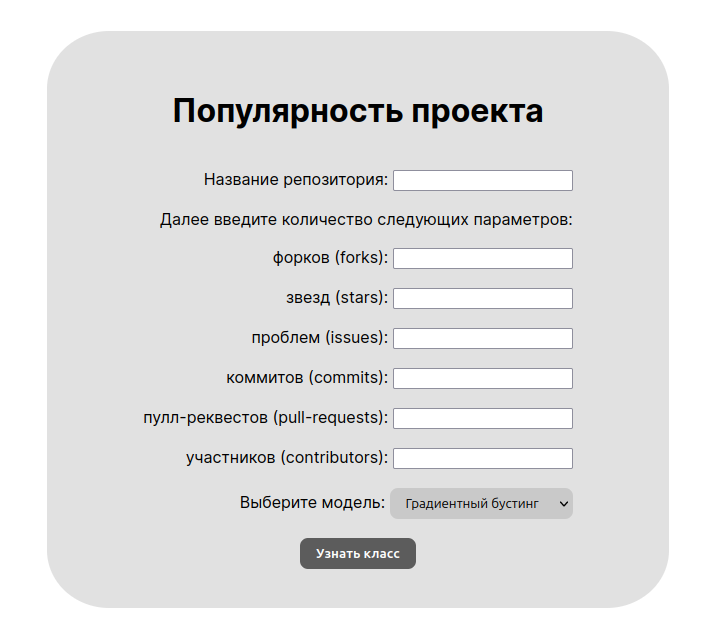
\includegraphics[scale=0.5]{pic/form-data.png}
        \caption{Форма для ввода данных}
        \label{ris:form-data}
    \end{figure}
\end{center}
\vspace{1.5em}

Кроме того, можно выбрать модель, на базе которой будет определен класс популярности проекта. После получения данные проходят обработку, и открывается страницу, на которой отображен результат определения полученного ранга с перечислением того, какие данные были отправлены (рис.~\ref{ris:result-data})

\begin{center}
    \begin{figure}[H]
        \center{\includegraphics[width=0.4\linewidth]{image}}
        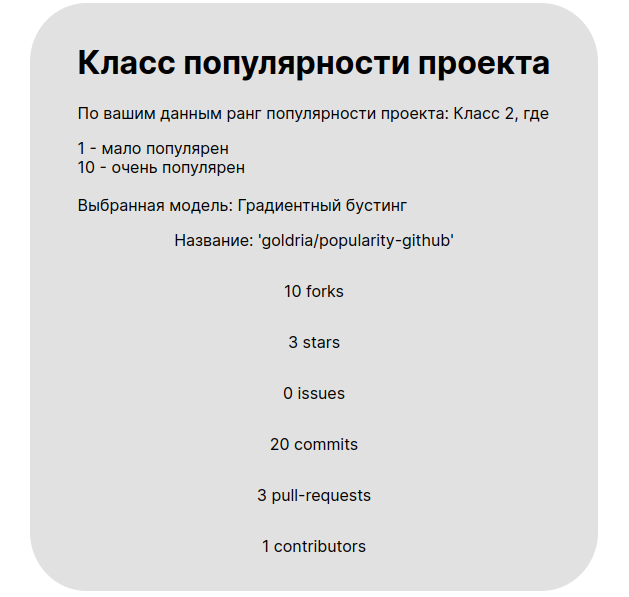
\includegraphics[scale=0.5]{pic/result-data.png}
        \caption{Форма для ввода данных}
        \label{ris:result-data}
    \end{figure}
\end{center}
\vspace{1.5em}